\chapter{Literature Review}
\label{chap:background}

%##################################################################################################
\section{Chapter Overview}
%##################################################################################################

In Chapter~\ref{chap:introduction}, the segmentation and feature identification problems were introduced, and my thesis was formally stated. This chapter surveys some of the wide variety of segmentation and feature identification techniques currently in use in the field of medical imaging, with the intention of providing the background necessary to place the specific techniques I used for my own work in context. It also surveys some of the uses of partition hierarchies (trees and forests) throughout computer science as a whole. This background lays the foundation for Chapter~\ref{chap:methodology}, in which the research approach I chose is discussed in the context of the overall goals of my doctoral work.

Whilst the segmentation and feature identification problems are theoretically distinct -- in that feature identification involves assigning semantic meaning to parts of an image where segmentation does not -- there is a great deal of overlap between them in practice. For example, the goal of some of the segmentation techniques we will see (e.g.~region growing) is to directly segment a particular feature of interest; in that sense, they are as much feature identification approaches as segmentation ones. For that reason, I have chosen to present the techniques used for both problems together, rather than separately.

The discussion of existing work on partition hierarchies foreshadows the formal definition of partition forests and the presentation of novel algorithms for working with them in Chapter~\ref{chap:ipfs}. Partition forests are a generalization of the partition trees that result from a certain type of bottom-up (merging-based) construction process, and the background on other areas where partition hierarchies are applied thus lays the groundwork for assessing the wider usefulness of my algorithms in Chapter~\ref{chap:assessment}.

%##################################################################################################
\section{Segmentation and Feature Identification}
%##################################################################################################

%################################################
\subsection{Overview}
%################################################

The majority of the segmentation techniques in current use can be divided into eight classes:

\begin{enumerate}

\item \emph{Thresholding techniques}, which seek to segment an image based on dividing up the histogram of its grey values.
\item \emph{Region growing techniques}, which search for specific features by flooding outwards from one or more initial seed points in the image.
\item \emph{Morphological techniques} such as the watershed transform, which treats an image as a height map and divides it up into catchment basins that we try to ensure correspond to features of interest.
\item \emph{Deformable models}, which start with some arbitrary model of a desired feature and try to deform it to fit the image data.
\item \emph{Learning techniques}, which construct some variety of model based on a set of training images and use it to segment subsequent scans.
\item \emph{Clustering techniques}, which try and cluster objects (in this case image pixels) into groups whose members are mutually similar, but dissimilar to the members of other groups.
\item \emph{Graph partitioning techniques} such as the normalized cuts algorithm.
\item \emph{Hybrid techniques}, which combine methods from the other classes to produce good results for specific applications.

\end{enumerate}

\noindent Each of these is discussed in more detail in one of the following subsections.

%################################################
\subsection{Thresholding}
%################################################

In principle, thresholding segmentation methods are quite simple. The idea is to divide the pixels of the image into classes through the use of one or more dividing lines on the image histogram. Dividing the image into two classes is known as \emph{binary thresholding}; where more classes are used, we refer to the process as \emph{multi-thresholding}. As an example, we could use binary thresholding to divide an 8-bit image (with grey levels ranging from $0 = \mbox{black}$ to $255 = \mbox{white}$) into two classes, one containing pixels greater than (say) $125$, and representing the foreground of the image, and the other containing all the remaining pixels and representing the background (see Figure~\ref{fig:background-segmentation-thresholding-binaryexample}). This would allow us to achieve the goal of segmenting the brighter object in the image.

%---
\begin{stusubfig}{p}
	\subfigure[The original image]
	{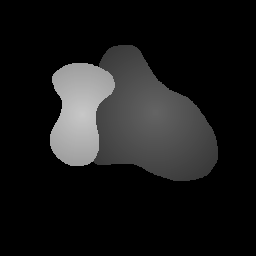
\includegraphics[height=.2\textheight]{background/background-segmentation-thresholding-binaryexample-a.png}}%
	%
	\hspace{4mm}%
	%
	\subfigure[The thresholded image]
	{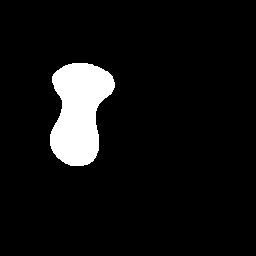
\includegraphics[height=.2\textheight]{background/background-segmentation-thresholding-binaryexample-b.png}}%
	%
	\hspace{4mm}%
	%
	\subfigure[The image histogram and threshold (at grey value $125$)]
	{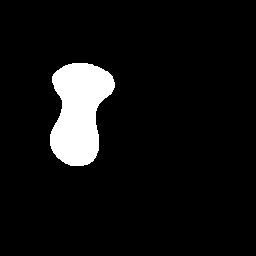
\includegraphics[height=.2\textheight]{background/background-segmentation-thresholding-binaryexample-c.png}}%
\caption{Segmenting the brighter of two adjacent objects in an 8-bit greyscale image using binary thresholding (the objects are easily separated in this case because the distribution of grey values in the image is bimodal)}
\label{fig:background-segmentation-thresholding-binaryexample}
\end{stusubfig}
%---

%---
\begin{stusubfig}{p}
	\subfigure[Segmenting Figure~\ref{fig:background-segmentation-thresholding-binaryexample}(a) with a threshold of $175$ undersegments the brighter object]
	{
\includegraphics[height=.2\textheight]{background/background-segmentation-thresholding-inaccurate-a.png}}%
	%
	\hspace{4mm}%
	%
	\subfigure[Conversely, segmenting the same image with a threshold of $75$ oversegments the brighter object]
	{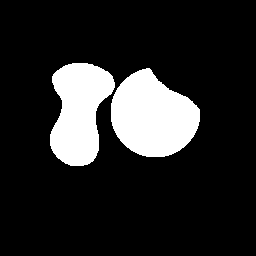
\includegraphics[height=.2\textheight]{background/background-segmentation-thresholding-inaccurate-b.png}}%
\caption{Misplaced thresholds lead to inaccurate segmentations}
\label{fig:background-segmentation-thresholding-inaccurate}
\end{stusubfig}
%---

\afterpage{\clearpage}

The difficulty encountered in practice is how to determine the optimum threshold location(s). A misplaced threshold will cause an inaccurate segmentation, so choosing the location appropriately is essential. In our example above, choosing a threshold that is too high will mean that the brighter object will be \emph{undersegmented} (i.e. some pixels which should be classified as being part of the foreground are incorrectly being classified as background) and the background will be \emph{oversegmented} (the converse) -- see Figure~\ref{fig:background-segmentation-thresholding-inaccurate}(a). Choosing too low a threshold will cause the opposite problem -- see Figure~\ref{fig:background-segmentation-thresholding-inaccurate}(b).

Owing to difficulties like this, applications are often designed so that thresholds can be chosen interactively by the user, but a great deal of work has also been done on automatically determining good threshold locations. As surveyed by Sezgin and Sankur in \cite{sezgin04}, there are six types of approach to the problem in current use:

\begin{enumerate}

\item \emph{Histogram shape-based methods.} These use shape properties of the histogram to find a good threshold. For instance, Rosenfeld's histogram concavity method, cited in \cite{lee.c92}, works by examining the difference between a histogram and its convex hull. A grey level at which the the height difference between the histogram and its convex hull is greatest (i.e. a point of deepest concavity) is picked as the threshold value.

\item \emph{Clustering-based methods.} These try and group the grey level data into a given number of clusters (two in the case of binary thresholding). One example is the method of Ridler and Calvard \cite{ridler78}. Their idea was to take a grey-level image and produce an initial binary classification which makes the assumption that the object of interest is somewhere in the middle of the image and the corners of the image contain only background. The means of the pixels currently classified as background and object are calculated and the average of the two means is taken. The new value is then used to threshold the image and produce a new binary classification into background and object classes: it is assumed that this will be more accurate than the initial guess. Finally, the process is iterated until there is little or no change in the binary classification, and the last threshold in the iteration is chosen for use.

\item \emph{Entropy-based methods.} These are based on information theory and pick thresholds by (for example) trying to maximise the information content in the thresholded image. As described by Wong and Sahoo in \cite{wong89}, the simplest possible such method looks at two probabilities, $F(T)$ and $F^*(T) = 1 - F(T)$, each parameterised in terms of a threshold, $T$. The first, $F(T)$, gives us the probability of a particular pixel having a grey value less than or equal to the threshold, and the second, $F^*(T)$, gives us the probability of the value being greater than it. The information content in the thresholded image is given by
%
\[
H(T) = -F(T) \log_2 F(T) - F^*(T) \log_2 F^*(T)
\]
%
and attains a maximum when $F(T) = 0.5$. This is equivalent to saying that in the absence of any other knowledge, the maximum entropy principle tells us that the information contained in the thresholded image is maximised by picking a threshold which classifies half the pixels as background and half as foreground. This makes intuitive sense, but is too simplistic an approach for the majority of applications. Better alternatives have been developed (see \cite{sezgin04}), but are beyond the scope of this dissertation.

\item \emph{Object attribute-based methods.} These pick thresholds based on a comparison between the original grey-level image and the binarized (i.e.~segmented into two classes) version of it. For example, the method of Hertz and Schafer \cite{hertz88} picks the threshold that yields a binarized image whose edge field maximally corresponds to that of the original image. The edge fields in this case are obtained via the well-known Sobel operator \cite{gonzalez02}.

\item \emph{Spatial methods.} An example of a spatial thresholding method is Wu et al.'s approach in \cite{wu82}. This first constructs a quadtree from the image by splitting image regions until they have a low standard deviation (where they define `low' in terms of the standard deviation of the image as a whole). This divides the image into square blocks of various different sizes. The observation is that the smaller blocks tend to be near the boundaries between foreground and background in the image -- the quadtree can thus be used as a way of estimating where these boundaries are. Having classified the pixels in the image in this way, it is possible to construct a histogram of the grey values of non-boundary pixels in the image, which it is hoped will be more bimodal than the histogram of the grey values in the image as a whole. A threshold can then be placed at the deepest point in the value between the two modes. Alternatively, a histogram of the boundary pixels can be constructed, which it is hoped will be unimodal, and a threshold can be placed at the mean of this histogram instead.

\item \emph{Local / adaptive methods.} These vary the threshold for each pixel location in the image. Two examples of this are the methods of Bernsen \cite{bernsen86} and Niblack \cite{niblack86}. As described by Trier and Jain in \cite{trier95}, Bernsen's method takes the highest and lowest grey values, $g_{\mbox{max}}$ and $g_{\mbox{min}}$, in a suitably-sized window around each pixel, and uses them to calculate a contrast measure $C = g_{\mbox{max}} - g_{\mbox{min}}$. If $C$ is less than some user-specified value, the local neighbourhood around the pixel is taken to be uniform, and an appropriate choice is made about whether the pixel should be classified as background or foreground (in \cite{trier95}, pixels were always classified as background in this case). Otherwise, a threshold value $T = (g_{\mbox{max}} + g_{\mbox{min}}) / 2$ is calculated, and the pixel is classified as foreground if its value is greater than $T$, and background if not. Niblack's method, by contrast, bases its decision on the mean and standard deviation of the grey values in the local neighbourhood around a pixel. In particular, if $m$ is the local mean and $s$ the local standard deviation, Niblack's method calculates a local threshold $T = m + ks$, where $k$ is a (negative) user-specified parameter. Again, a pixel is classified as foreground iff its grey value is greater than $T$.

\end{enumerate}

%---
\begin{stusubfig}{p}
	\subfigure[An example CT image]
	{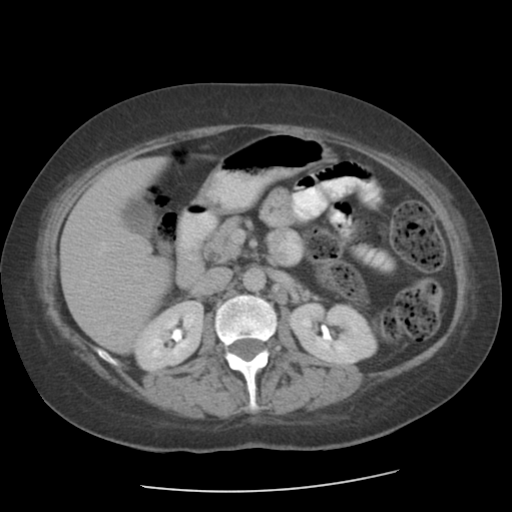
\includegraphics[width=.45\linewidth]{background/background-segmentation-thresholding-ct-a.png}}%
	%
	\\
	%
	\subfigure[{The results of trying to segment the kidneys using thresholding with a foreground range of $[160,215]$}]
	{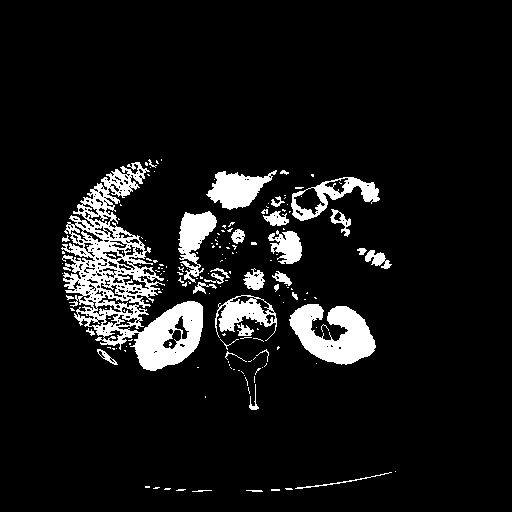
\includegraphics[width=.45\linewidth]{background/background-segmentation-thresholding-ct-b.png}}%
	%
	\hspace{4mm}%
	%
	\subfigure[{The results of trying to segment the kidneys using thresholding with a foreground range of $[175,195]$}]
	{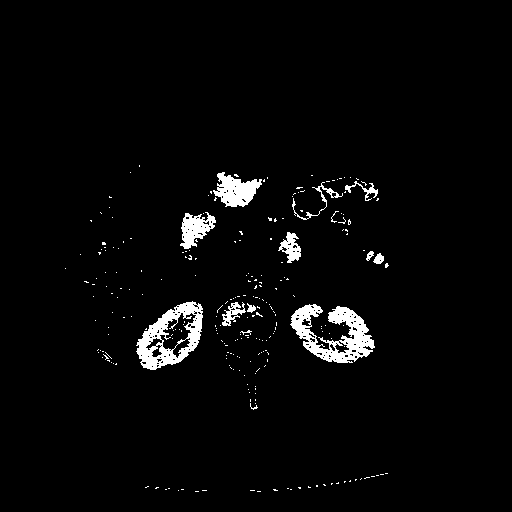
\includegraphics[width=.45\linewidth]{background/background-segmentation-thresholding-ct-c.png}}%
\caption{Trying to segment the kidneys in the CT image in (a) using thresholding alone doesn't work. If we choose a wide foreground range, as in (b), we oversegment the kidneys, dragging in lots of unrelated features across the image. If we choose a narrower range to try and prevent this, as in (c), we miss pieces of the kidneys themselves and end up with holes. Note that even in (c), we are unable to prevent other features being segmented as well as the kidneys, as the grey value distributions of the kidneys and other features overlap.}
\label{fig:background-segmentation-thresholding-ct}
\end{stusubfig}
%---

\noindent In spite of the large amount of work done on thresholding, however, it has some significant downsides when used on its own to process more complicated images:

\begin{itemize}

\item It is by no means the case that acceptable threshold locations always exist. If the grey value ranges of different objects of interest significantly overlap, it may be impossible to isolate individual features using thresholding alone. Consider trying to segment the kidneys, as in Figure~\ref{fig:background-segmentation-thresholding-ct}, by bounding them between two grey value thresholds. If we choose too wide a foreground range, as in (b), we succeed in segmenting the kidneys, but end up inadvertently including other features (bits of the liver, aorta, etc.); if we choose a narrower foreground range to try and avoid this, as in (c), we succeed to some extent in reducing this oversegmentation, but the resulting kidneys now contain holes. There is in fact no range that we can choose that will not suffer from either problem, as the grey values that must be in our range in order to segment the kidneys are shared by other features in the image.

\item There is no guarantee (or even an expectation) that any of the groups of pixels into which thresholding divides the image will be contiguous. When a wide foreground range is chosen (as in Figure~\ref{fig:background-segmentation-thresholding-ct}(b)), it is thus common to end up segmenting lots of separate foreground regions across the entire image that only have grey values in common. Conversely, when a narrow foreground range is chosen (as in Figure~\ref{fig:background-segmentation-thresholding-ct}(c)), the segmented result usually contains the aforementioned holes, corresponding to lots of separate background regions that only have grey values in common. As shown in Figure~\ref{fig:background-segmentation-thresholding-ct}(c), it is in fact possible to suffer from both these problems at once.

\end{itemize}

\noindent Thresholding's limitations can in some cases be overcome by combining thresholding with other techniques. For instance, whilst the results of thresholding often have holes in them, these can sometimes be filled in by carefully applying a technique called morphological closing (the graph-based version of which is described in Chapter~\ref{chap:featureid}). Where thresholding has produced lots of small regions across the image, it is sometimes possible to remove them and keep only the larger ones by using connected component analysis. Luc Soler's team \cite{soler01} made use of thresholding (as one technique among many) and achieved excellent automatic segmentation results for the liver. However, they did not use thresholding on its own. For instance, they segmented bones by thresholding for bright areas and then keeping only those which were near to the fat tissue (which had already been segmented). Simple thresholding alone would have been insufficient for the task, since structures such as the aorta also appeared bright on the contrast-enhanced images.

%################################################
\subsection{Region Growing}
\label{subsec:background-segmentation-regiongrowing}
%################################################

Region growing methods for segmentation essentially work as follows. First, one or more initial seed points are chosen for a feature of interest. Then, the region is `grown' by iteratively considering all points which are adjacent to those already in the region and adding any which satisfy certain criteria (see Figure~\ref{fig:background-segmentation-regiongrowing-process}). For example, we could choose to add adjacent pixels whose grey value differs from that of their neighbour in the region by less than a certain amount. Alternatively, we could try and add adjacent pixels which preserve the homogeneity of the entire region (for some suitable definition of homogeneity) -- e.g.~Chen et al.\ \cite{chen09} define a criterion that leads an adjacent pixel to be added to the region provided that the absolute difference between its grey value and the mean grey value of the region is less than the standard deviation of the region's grey value distribution.

%---
\begin{stusubfig}{p}
	\subfigure[Initial state]
	{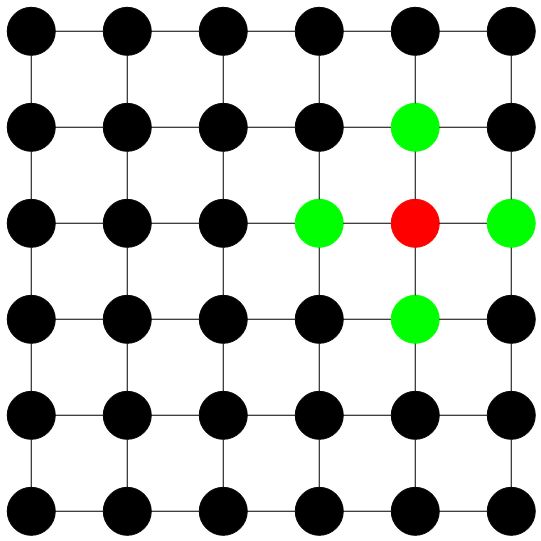
\includegraphics[height=4.5cm]{background/background-segmentation-regiongrowing-process-a.png}}%
	%
	\hspace{12mm}%
	%
	\subfigure[After one iteration]
	{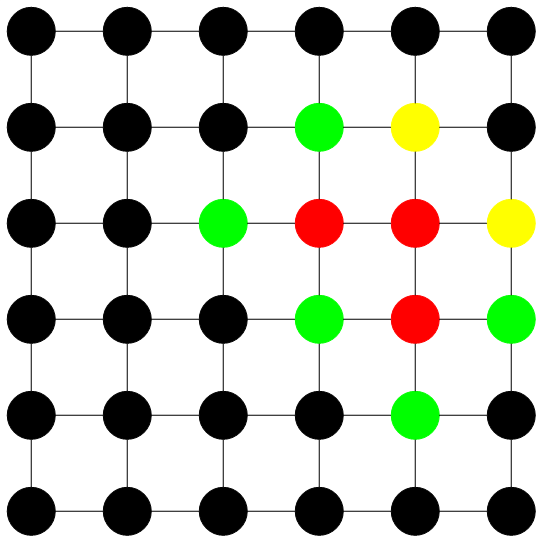
\includegraphics[height=4.5cm]{background/background-segmentation-regiongrowing-process-b.png}}%
	%
	\\ \vspace{4mm}
	%
	\subfigure[After two iterations]
	{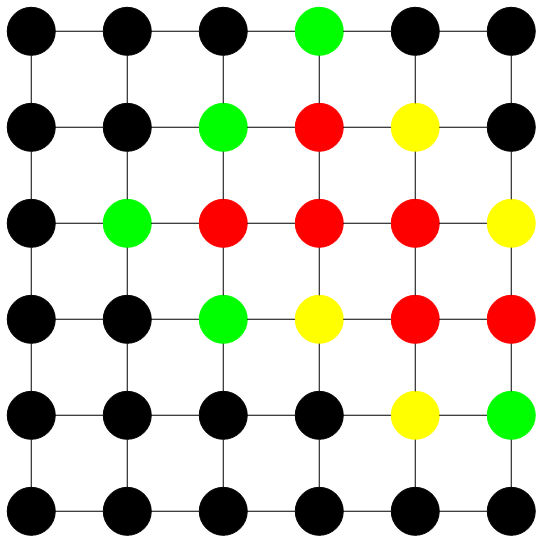
\includegraphics[height=4.5cm]{background/background-segmentation-regiongrowing-process-c.png}}%
	%
	\hspace{12mm}%
	%
	\subfigure[Final state]
	{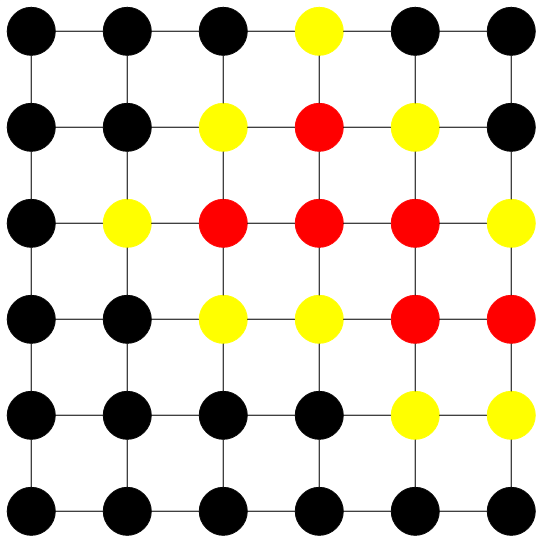
\includegraphics[height=4.5cm]{background/background-segmentation-regiongrowing-process-d.png}}%
\caption{An example region growing process -- black pixels are those not yet considered, red pixels are those currently in the region, green pixels are those under consideration, and yellow pixels are those that already failed the similarity criterion. The algorithm terminates when there are no further pixels to consider. The final segmented object is shown in red in (d).}
\label{fig:background-segmentation-regiongrowing-process}
\end{stusubfig}
%---

%---
\begin{stulisting}[p]
\caption{A Generic, Single-Seed Region Growing Algorithm}
\label{code:background-segmentation-regiongrowing-generic}
\begin{lstlisting}[style=Default]
function grow_region
: (seed : PixelCoords; criterion : PixelCoords $\to$ bool) $\to$ Set<PixelCoords>

	var queue : Queue<PixelCoords>;
	var result, visited : Set<PixelCoords>;

	// Add the seed point to the queue and mark it as visited.
	queue.push(seed);
	visited.insert(seed);

	while not queue.empty()
		p := queue.pop();
		result.insert(p);

		// Add neighbours satisfying the similarity criterion to the queue.
		for each neighbour $\in$ neighbours(p)
			if not visited.contains(neighbour) then
				if criterion(neighbour) = true then queue.push(neighbour);
				visited.insert(neighbour);
			
	return result;
\end{lstlisting}
\end{stulisting}
%---

More involved criteria are also possible. One popular approach is that of \emph{adaptive} region growing (e.g.~see \cite{lin06,pohle01}), whereby the criterion varies to take account of the area around the pixel under consideration. In \cite{lin06}, for example, the approach taken is as follows. After locating an initial seed point $(s_x, s_y)$, a $7 \times 7$ mesh is placed over it and the maximum and minimum pixel intensities within the mesh, $M(s_x, s_y)$ and $m(s_x, s_y)$ are determined. From these, a contrast range $t_0 = M(s_x, s_y) - m(s_x, s_y)$ is calculated and recorded. Next, for each pixel $(x,y)$ under consideration for addition to the region, values $M(x,y)$ and $m(x,y)$ are similarly calculated, and a local value $\theta_{\rm local} = (M(x,y) + m(x,y)) / 2$ is determined. The region growing criterion is then formulated as $|f(x,y) - \theta_{\rm local}| \le t_0$, i.e. we add an adjacent pixel $(x,y)$ to the region if the absolute difference between its grey value $f(x,y)$ and the midpoint of the contrast range of the $7 \times 7$ mesh surrounding it is less than the contrast range of the $7 \times 7$ mesh centred on the initial seed point. The region growing is specified to stop when this absolute difference is greater than a certain threshold, implying that the area surrounding a given pixel is not homogeneous.

A generic, single-seed region growing algorithm can be implemented straightforwardly using a queue (see Listing~\ref{code:background-segmentation-regiongrowing-generic}). Starting from a queue containing only the initial seed point, we repeatedly pop the pixel at the front of the queue, consider its non-region neighbours for addition to the region, and push any which satisfy the requisite criteria onto the end of the queue. The process terminates when the queue empties.

The key policy issues to consider when implementing region growing are how to choose the seed points, how to formulate the criteria specifying which points to add to the region, and how to decide when the process should terminate. For automated segmentation methods, how to choose the seed points is of fundamental importance; semi-automated algorithms can focus exclusively on the latter two problems, relying instead on the user to interactively specify any initial seeds.

%---
\begin{stusubfig}{p}
	\subfigure[An example CT image, with seeds marked at $(150,360)$ and $(350,340)$]
	{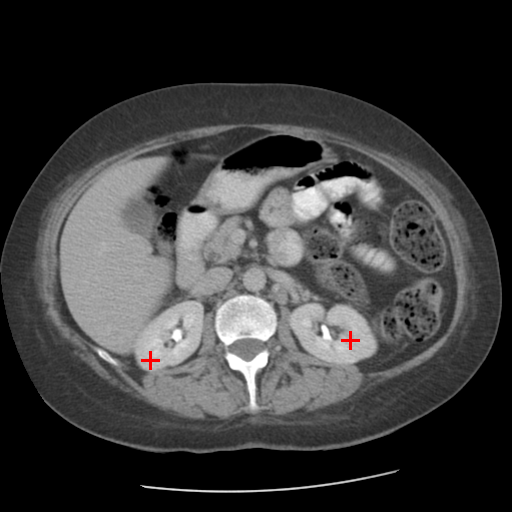
\includegraphics[width=.45\linewidth]{background/background-segmentation-regiongrowing-ct-a.png}}%
	%
	\hspace{4mm}%
	%
	\subfigure[{The results of trying to segment the kidneys using region growing -- the grow condition specifies that adjacent pixels are added if their grey values are in the range $[165,215]$}]
	{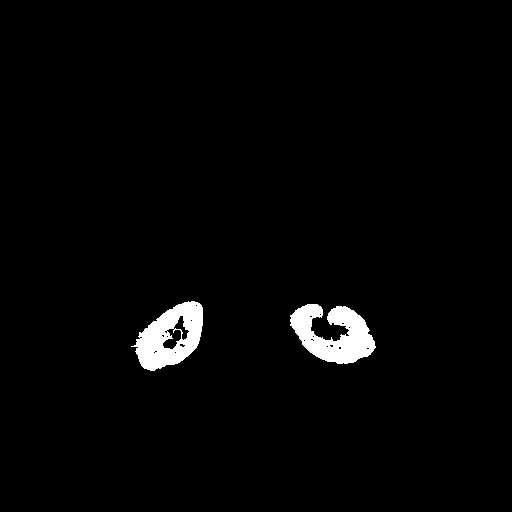
\includegraphics[width=.45\linewidth]{background/background-segmentation-regiongrowing-ct-b.png}}%
\caption{Segmenting features using region growing can be very effective, but it relies on the user to specify seed points and a sensible grow condition}
\label{fig:background-segmentation-regiongrowing-ct}
\end{stusubfig}
%---

%---
\stufigex{height=8cm}{background/background-segmentation-regiongrowing-lin.png}{The candidate regions searched for kidney seeds in \cite{lin06} (reproduced from the paper in question)}{fig:background-segmentation-regiongrowing-lin}{p}
%---

The advantages of region growing methods are that the segmentation result is guaranteed to have no more connected components than there were initial seeds (thus, single-seed methods are guaranteed to produced a connected result), and that they are, on the whole, fairly easy to implement. An example of the sort of results that can be achieved is shown in Figure~\ref{fig:background-segmentation-regiongrowing-ct}. However, from the point of view of automatic segmentation, they present difficulties, because choosing initial seed points automatically is in general a non-trivial problem. The usual approach taken for automatic seed point selection is to rely on statistical data about where the features of interest (e.g. organs) usually lie in the body. For instance, the approach in \cite{lin06} was to search for suitable seed points in two elliptical regions on each side of the body, one for each kidney (see Figure~\ref{fig:background-segmentation-regiongrowing-lin}). This worked quite well in context, but is not robust in the general case, relying strongly on the kidneys being in the expected places -- for example, it is unsuitable for MRI images, in which the patient's body may be oriented arbitrarily. It would also fail if used for images of auto-transplant patients.\footnote{Auto-transplantation involves transplanting an organ, or part of an organ, from one part of a patient's body to another. For instance, partial nephrectomy operations (which involve cutting away part of a kidney) are sometimes performed by removing the kidney, cutting away the relevant piece outside the body, and then reimplanting what is left of the kidney.}

Whilst region growing algorithms produce connected regions around each seed, each region may still have holes in the middle of it. Whilst this may be desirable if we really are trying to segment torus-shaped features, on the whole it is necessary to post-process the region growing results to remove these holes, e.g.~using morphological closing.

%################################################
\subsection{Morphological Techniques}
\label{subsec:background-segmentation-morphology}
%################################################

Mathematical morphology is a large and rather general field based on lattice theory \cite{goutsias00}. It contains many useful image processing techniques, including the morphological operators of which we will see graph-based versions in Chapter~\ref{chap:featureid}, but in segmentation terms its key technique is the watershed transform, originally developed by Serge Beucher \cite{beucher90}.\fxnote{[IDV] [The morphological techniques section needs an image-based example]}

The watershed, which will be described in substantially more detail in Chapter~\ref{chap:segmentation}, is essentially a technique for dividing landscapes into their catchment basins (where a catchment basin is an area of the landscape from which water would run down to a given local minimum) -- see Figure~\ref{fig:background-segmentation-watershed-concept}. In imaging terms, this can be utilised for segmentation purposes by treating an image as a discrete landscape and pre-processing it so as to try to establish a correspondence between catchment basins in the landscape and features of interest in the image. If such a correspondence can be successfully established, finding the catchment basins then equates to finding the desired image features.

%---
\stufigex{width=8cm, height=8cm}{segmentation/segmentation-watershed-concept.png}{The watershed transform constructs watersheds (the red partitions) that divide a landscape into its catchment basins}{fig:background-segmentation-watershed-concept}{p}
%---

Many image algorithms have been developed to actually perform the watershed transform; in general, these can be classified as either flooding algorithms (e.g.~\cite{bieniek00,rambabu07}) or rainfalling algorithms (e.g.~\cite{meijster98,osma-ruiz06,stoev00}). The former essentially flood out from the local minima in the landscape and (implicitly or otherwise) add watershed boundaries where the different catchment basins meet; the latter determine paths of steepest descent from points in the landscape and assign them to catchment basins based on the local minima to which their paths lead down.

In practice, however, it is rarely possible to establish a perfect correspondence between the catchment basins in the landscape and the desired features in the image, as to do so consistently would require prior knowledge of where the desired features actually are in the image, which would defeat the point of segmenting the image in the first place. One of the most common problems encountered with the watershed transform is that of oversegmentation: the landscape fed into the watershed has an excess number of catchment basins, most of which do not correspond to anything of interest in the actual image (see Figure~\ref{fig:background-segmentation-watershed-normal}). This is particularly true of landscapes representing noisy images -- small changes in grey values can create shallow catchment basins, or dimples, in the landscape, greatly affecting the resulting segmentation.

%---
\begin{stusubfig}{p}
	\subfigure[]
	{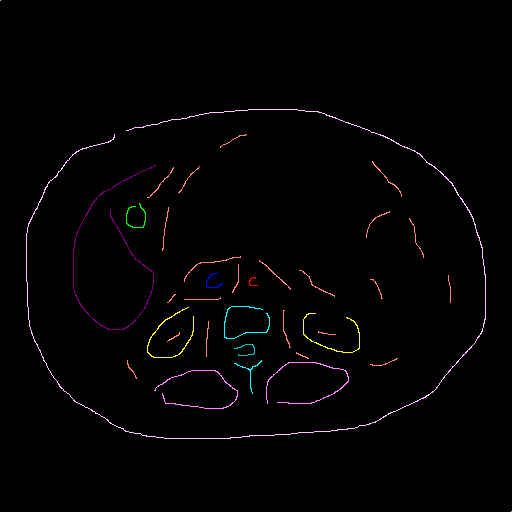
\includegraphics[width=.4\linewidth]{background/background-segmentation-watershed-markers-a.png}}%
	%
	\hspace{4mm}%
	%
	\subfigure[]
	{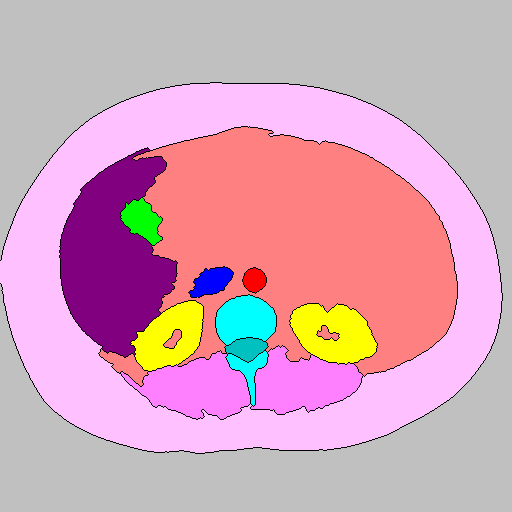
\includegraphics[width=.4\linewidth]{background/background-segmentation-watershed-markers-b.png}}%
\caption{The watershed-from-markers technique can be used to solve the oversegmentation problem that plagues the normal watershed, but it can require a significant amount of user input, making it unsuitable for use as an \emph{automated} segmentation method. Here, watershed-from-markers is provided with a user-specified marker image (a) and used to segment the gradient magnitude image from Figure~\ref{fig:background-segmentation-watershed-normal}(b). The result (b) is relatively good, but only because the marker image provides the algorithm with far more information than it would have without user involvement. Generating such a marker image automatically is non-trivial.}
\label{fig:background-segmentation-watershed-markers}
\end{stusubfig}
%---

%---
\begin{stusubfig}{p}
	\subfigure[]
	{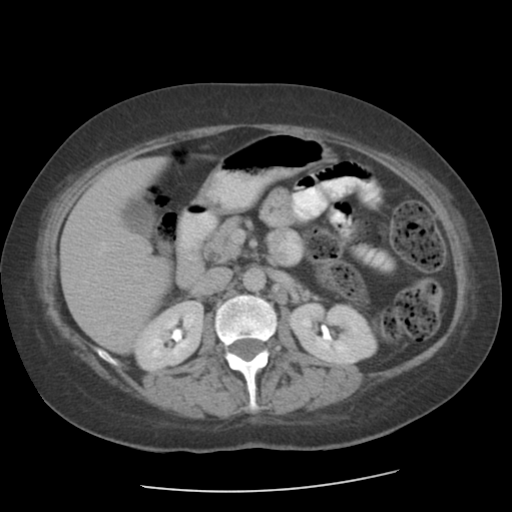
\includegraphics[width=.45\linewidth]{background/background-segmentation-watershed-normal-a.png}}%
	%
	\hspace{4mm}%
	%
	\subfigure[]
	{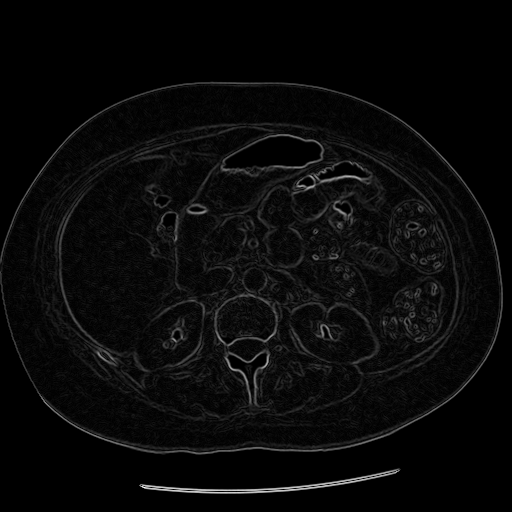
\includegraphics[width=.45\linewidth]{background/background-segmentation-watershed-normal-b.png}}%
	%
	\\ \vspace{4mm}
	%
	\subfigure[]
	{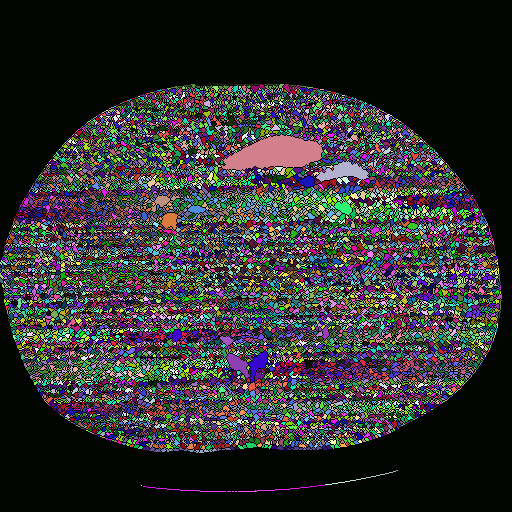
\includegraphics[width=.45\linewidth]{background/background-segmentation-watershed-normal-c.png}}%
\caption{Running a normal watershed on an image tends to produce an oversegmented result. Here, an example CT image (a) is first passed through a gradient magnitude filter to try and establish more of a correspondence between catchment basins and features (b). A watershed transform is then performed on the gradient magnitude image, producing a significant oversegmentation due to the large number of spurious catchment basins in the landscape (c). A few larger regions, such as part of the stomach, have been successfully segmented, because their pixels share a single grey value in the image, but the rest of the segmentation is clearly inadequate without further processing.}
\label{fig:background-segmentation-watershed-normal}
\end{stusubfig}
%---

There are two main approaches in the literature for dealing with this problem, namely marker imposition (leading to an approach known rather aptly as `watershed-from-markers') and hierarchical segmentation. Marker imposition essentially works by specifying markers on particular features of interest \emph{a priori}, and flooding out only from those. This partitions an image into a number of regions equal to the number of specified markers and thereby solves the oversegmentation problem (see Figure~\ref{fig:background-segmentation-watershed-markers}). Unfortunately, it can be extremely difficult to determine the required markers automatically -- rather than solving the underlying problem, we have merely changed it into one of marker determination. This may or may not prove problematic, depending on the data available and the specifics of the application. In some cases, it may be possible to use other data to determine marker placement automatically -- for example, Grau et al.\ \cite{grau04} successfully used a statistical atlas for this. In other cases, it may simply be acceptable to place the markers manually \cite{xue05}, or to initially place them manually and then propagate them from one image in a sequence to the next \cite{flores09}.

In situations where neither is the case, however, the alternative approach of hierarchical segmentation can be used. As one might expect, the general idea here is to take the oversegmented result of running the watershed transform on an image, and perform several iterations of region merging to produce a hierarchy of gradually coarser partitions of the original image. As will be illustrated in far more detail in Chapter~\ref{chap:segmentation}, this is exactly the sort of approach taken by the waterfall transform \cite{beucher90,marcotegui05}: what is unique about the waterfall, however, is that each of its iterations in which it merges regions together is itself a watershed transform.

As will be discussed in Chapter~\ref{chap:methodology}, the hierarchical approach to watershed segmentation is interesting for a couple of reasons: on the one hand, it produces, without requiring a great deal of manual fine-tuning, segmentations which, whilst not perfect, are often quite reasonable to a first approximation; on the other hand, the hierarchy of partitions of the image it produces can be turned into a tree structure (see \S\ref{sec:background-partitionhierarchies}) that is amenable to further editing, allowing any flaws in the initial segmentation to be corrected in an intuitive manner. These two qualities make this approach eminently suitable in situations where automated solutions are desirable but interactive control remains important.

%################################################
\subsection{Deformable Models}
%################################################

As their name suggests, deformable models methods work by taking an initial model of the features under consideration and deforming it to fit the actual data available. The initialisation of the model is generally based on \emph{a priori} anatomical knowledge. The model itself can be represented in a variety of ways, and these ways correspond to a number of different approaches to the problem. For example, the snakes method, which we will see shortly, represents the model as a parametrically-defined spline, and is hence referred to as an example of a parametric deformable model (it is sometimes also referred to as an explicit deformable model). In contrast, level sets represent the model \emph{implicitly} and are an example of implicit deformable models. Implicit deformable models were developed later than their parametric counterparts, but both types see a lot of use.

%~~~~~~~~~~~~~~~~~~~~~~~~~~~~~~~~~~~~~~~~~~~~~~~~
\subsubsection{Parametric Deformable Models}
%~~~~~~~~~~~~~~~~~~~~~~~~~~~~~~~~~~~~~~~~~~~~~~~~

\paragraph{Snakes}

As originally defined by Kass, Witkin and Terzopoulos in \cite{kass88}, `A snake is an energy-minimizing spline guided by external constraint forces and influenced by image forces that pull it toward features such as lines and edges.' Essentially, the idea works as follows. We represent the position of the snake, in terms of a spline parameter $s$, as $\mathbf{v}(s) = (x(s),y(s))$, and define an \emph{energy functional}, $E_{snake}^*$, as
%
\[
E_{snake}^* = \int_0^1 E_{int}(\mathbf{v}(s)) + E_{image}(\mathbf{v}(s)) + E_{con}(\mathbf{v}(s)) \; ds.
\]
%
The three terms in the summation are \emph{internal} energy, which tries to limit the curvature of the snake, \emph{image} energy, which tries to attract the snake towards features in the image such as lines and edges, and \emph{constraint} energy, which allows the user to apply constraints to influence the result of the segmentation. The snake algorithm as a whole attempts to find a spline minimising $E_{snake}^*$.

The original snakes paper describes a continuous model, but more recent research \cite{lobregt95,miller90b,miller90a} has seen the development of discrete models as well. The model described by Lobregt and Viergever in \cite{lobregt95}, called a \emph{discrete dynamic contour model}, is particularly interesting, and worth describing in more detail. Rather than relying on ideas of energy-minimization, Lobregt and Viergever model snakes using a force-based physical simulation. In their approach, a snake is a set of vertices connected by edges. At each time-step, various forces are applied to each vertex, which gradually \emph{deform} the snake towards the desired result. The results of this approach will depend to an extent on the lengths of the edges joining the vertices: if an edge is too long, important image features may pass through the gaps between vertices; if it is too short, the snake may become overly fixated on small details, not to mention the speed of the process being adversely affected. For this reason, after each deformation step, the snake is \emph{resampled} (by adding or removing vertices where necessary) to keep the edge lengths within certain limits.

The forces applied to each vertex closely mimic the energy terms in the original snakes paper. The force $\mathbf{f_i}$ applied to vertex $i$ is defined as the weighted sum
%
\[
\mathbf{f_i} = w_{ex}\mathbf{f_{ex,r_i}} + w_{in}\mathbf{f_{in,i}} + \underbrace{w_{damp}}_{< \; 0}\mathbf{v_i},
\]
%
where $\mathbf{f_{ex,r_i}}$ is an \emph{external} force term corresponding to the image and constraint terms from the original formulation, $\mathbf{f_{in,i}}$ is an \emph{internal} force term corresponding to the original internal term, and the remaining term is a new addition used to apply damping to try and bring the simulation to rest. (The real numbers $w_{ex}$, $w_{in}$ and $w_{damp}$ specify the weights to be given to each of these three factors. The paper tended to set all three of these to $0.5$: apparently this was derived empirically.)

It is important to mention that the method relies on quite a close initialisation (i.e.~image features have quite a short capture range). In \cite{ree05}, this problem is circumvented by peforming a watershed-from-markers segmentation and using the result of that to initialise the snake. Another alternative, referred to there, is to try and add additional external forces to solve the problem: in particular, some success has been had with \emph{balloon forces} \cite{cohen91} and \emph{gradient vector flow} (GVF) \cite{xu98}. For example, Figure~\ref{fig:background-segmentation-snakes-gvfexample} shows a GVF snake successfully segmenting the left ventricle of a human heart.

%---
\stufigex{height=9cm}{background/background-segmentation-snakes-gvfexample.png}{The basic snakes method suffers from a poor capture range, but techniques such as gradient vector flow \cite{xu98} can mitigate this -- the figure (reproduced from the paper in question) shows a GVF snake deforming from an initial, circular contour to segment the left ventricle of a human heart }{fig:background-segmentation-snakes-gvfexample}{p}
%---

Problems of this kind with snakes methods have led to a great deal of interest in level sets as an alternative, although snakes also remain popular as a well-established and far simpler alternative. They also have the advantage that they can represent open structures as well as closed ones.

\paragraph{NURBS-Based}

Another type of parametric deformable model, this time based on non-uniform rational B-splines (NURBS), is described by Tsagaan et al.\ \cite{tsagaan02}, in which they use a 3D NURBS-based model of a kidney and deform it by minimizing an energy function. Their results seem good in some cases, but differ markedly from the manually segmented results they show in others.\fxnote{[IDV] [The heading isn't clear until you read the paragraph after it]}

%~~~~~~~~~~~~~~~~~~~~~~~~~~~~~~~~~~~~~~~~~~~~~~~~
\subsubsection{Implicit Deformable Models}
%~~~~~~~~~~~~~~~~~~~~~~~~~~~~~~~~~~~~~~~~~~~~~~~~

\paragraph{Level Sets}

Curves and surfaces in general can be specified either explicitly (such that they can be calculated directly from the definition) or implicitly (the opposite). For instance, an explicit (parametric) representation of a circle in terms of its radius $r$ and an angle $\theta$ might be:
%
\begin{eqnarray*}
x & = & r \cos \theta \\
y & = & r \sin \theta
\end{eqnarray*}
%
The corresponding implicit representation would be:
%
\[
x^2 + y^2 = r^2
\]
%
As we have seen, parametric deformable model approaches like snakes represent their model using the former approach. Level set approaches, by contrast, use the latter. As an introduction to the ideas behind level sets, consider the function $\psi(x,y) = x^2 + y^2$, which defines a scalar field over $\mathbb{R}^2$. For any value $k > 0$, the equation $\psi(x,y) = k$ defines a circle in the x-y plane: we will refer to each of these circles as an \emph{isosurface} of $\psi$, because each of them is the surface (curve) of all the points at which $\psi$ takes a particular value.\footnote{\emph{Iso} means `equal' in Greek, so here we are talking about the surface containing all the points with the same $\psi$ value.} The key idea is that if we now change $\psi$, for instance by redefining it as $\psi(x,y) = x^3 + y^3$, the isosurfaces change, in this case from circles to hypercircles. Thus, by changing the function $\psi$, we can move the isosurfaces of $\psi$ around without ever having to represent them explicitly. Level set approaches make use of this by representing the deformable model as an isosurface of some function $\psi$, and then modifying $\psi$ to deform the model towards the boundary of the desired image feature.

%---
\stufigex{height=5.5cm}{background/background-segmentation-levelsets-circleexample.png}{A simple circular contour which gradually expands over time}{fig:background-segmentation-levelsets-circleexample}{p}
%---

%---
\stufigex{height=5.5cm}{background/background-segmentation-levelsets-ellipseexample.png}{An example of a contour which changes its shape over time}{fig:background-segmentation-levelsets-ellipseexample}{p}
%---

%---
\stufigex{height=5.5cm}{background/background-segmentation-levelsets-uniformgrid.png}{Approximating a function $\psi(\mathbf{x},t)$ with a discrete, uniformly-spaced grid (note that the time superscripts on the grid values are not shown)}{fig:background-segmentation-levelsets-uniformgrid}{p}
%---

To represent contour changes over time, level set approaches make $\psi$ a function of time as well, and define it over some domain $U \subset \mathbb{R}^N$, giving us $\psi(\mathbf{x}, t) : U \times \mathbb{R}^+ \rightarrow \mathbb{R}$. They then set this equal to some constant (generally $0$) to actually specify one of the isosurfaces of $\psi$ as the contour being deformed. As a simple example of this, consider a circle, centred at the origin, which gradually expands outwards as the time increases (see Figure~\ref{fig:background-segmentation-levelsets-circleexample}). Supposing its radius to be $t$ at time $t$, we could represent this as:
%
\[
\psi((x,y),t) = x^2 + y^2 - t^2 = 0
\]
%
A more complicated example might involve gradually changing the circle into an ellipse over time (see Figure~\ref{fig:background-segmentation-levelsets-ellipseexample}). This could be achieved by writing:
%
\[
\psi((x,y),t) = x^2 + (yt)^2 - t^2 = 0
\]
%
Thus far, we have examined the basic ideas underpinning level sets, but not seen how they can be applied to the practical problem of segmentation. A common approach of real-world level set methods is to take as input not an explicit function of the kind we have just seen, but an initial contour on the image. This will then be deformed (using numerical methods) over time to try and fit it to an image feature of interest. There are thus six essential questions to consider:

\begin{enumerate}

\item How do we represent the function $\psi$?

\item Given an initial contour by the user, how do we use it to construct the initial function $\psi(\mathbf{x}, t = 0)$?

\item How do we define a numerical method to deform the initial function over time?

\item How do we know when the algorithm has terminated?

\item How do we extract the contour of interest over time?

\item How do we try and make the algorithm segment the desired image feature?

\end{enumerate}

\noindent To answer these questions, we consider the level set approach of Malladi et al., described in \cite{malladi95}. There, as tends to be the case for level set approaches in general, the function $\psi$ is represented by storing a discrete grid of approximate values over the domain $U$. The grid is uniformly-spaced, with squares of side $h$ (see Figure~\ref{fig:background-segmentation-levelsets-uniformgrid}). Each grid node has (for each integer value of $n \ge 0$) an associated value $\psi_{ij}^n$, which approximates the value $\psi((ih,jh),n\dt)$, where $\dt$ is the time step of the numerical method that will be used to deform the initial contour over time.

The initial goal is to construct, from a contour specified by the user, the grid of values $\psi_{ij}^0$ approximating the function $\psi(\mathbf{x},0)$. In \cite{malladi95}, this is done by setting $\psi_{ij}^0$ to be the signed distance of the grid node $ij$ from the initial contour (points outside the contour are assigned positive values and those inside are assigned negative ones) -- see Figure~\ref{fig:background-segmentation-levelsets-initialfunction}.

%---
\stufigex{height=5.5cm}{background/background-segmentation-levelsets-initialfunction.png}{Generating the initial function from the zero contour specified by the user (in red)}{fig:background-segmentation-levelsets-initialfunction}{p}
%---

Having constructed the grid for the initial function, the next step is then to define an appropriate numerical method to deform it over time. To do this, we first need a partial differential equation for $\psi$. The appropriate PDE, as derived in \cite{malladi95}, is:
%
\[
\pd{\psi}{t} + F|\nabla \psi| = 0
\]
%
Here, $F$ is called the \emph{speed function}, and will be used to control how $\psi$ evolves in a manner that will be discussed below. This can be approximated numerically as
%
\[
\frac{\psi_{ij}^{n+1} - \psi_{ij}^n}{\dt} + (F)(\nabla_{ij} \psi_{ij}^n) = 0,
\]
%
where (as noted, and described in more detail, in the paper), $\nabla_{ij} \psi_{ij}^n$ is `some appropriate finite difference operator for the spatial derivative'. This equation can be iteratively solved using standard numerical techniques (e.g.~see \cite{morton05}) and used to deform the model over time. The algorithm terminates when the contour of interest no longer changes between iterations.

To extract the contour of interest after each iteration, Malladi et al. construct a piecewise linear approximation to it, the gist of which involves finding the squares where some of the corner values are positive and some are negative, and constructing line segments therein. This bears not a little resemblance to the marching squares algorithm, the 2D analogue of marching cubes \cite{lorensen87}.

The remaining issue is how to use this algorithm to actually segment features in an image. For this, we make use of the speed function $F$, which controls how the contour deforms. Malladi et al.\ go into great detail about how $F$ should be defined, but essentially the idea is to define it so as to have (a) an advection component -- basically a term providing a constant speed inwards or outwards, (b) an image component -- a term which tries to make the contour move quickly when it is not near potential feature boundaries and slowly when it is close to them, and possibly (c) a geometry component -- a term which aims to control the local curvature of the contour. For the two-component version, with only an advection and an image component, this corresponds to an equation of the form
%
\[
\pd{\psi}{t} + (F_A + \hat{F}_I)|\nabla \psi| = 0,
\]
%
where $F_A$ is the advection component and $\hat{F}_I$ is the image component. For the version with a geometry component as well, the equation becomes
%
\[
\pd{\psi}{t} + \hat{k}_I(F_A + F_G)|\nabla \psi| = 0,
\]
%
where $F_G$ is the geometry component and $\hat{k}_I$ fulfils the role of the image component in the previous equation. The detailed definitions of the various components can be found in \cite{malladi95}. It is worth noting that this term-based approach bears a lot of similarity to that used for snakes, and in general the motivations for the various terms are more or less the same in each case.

Level sets have a number of advantages over snakes. One advantage is that they handle topological changes in an extremely simple fashion. For instance, consider Figure~\ref{fig:background-segmentation-levelsets-topologychanges}(a), in which the isosurface $\psi = 4$ is divided into two separate components. This is seamlessly represented by a level set approach, since it merely has to maintain a grid of numbers and not one or more explicit curves. Furthermore, the number of components can evolve over time without any special handling being required: in Figure~\ref{fig:background-segmentation-levelsets-topologychanges}(b), a change to the value of a single grid point can merge the two separate components into one, changing the topology at a stroke without any fuss. A corresponding implementation with snakes would involve far more work.

%---
\begin{stusubfig}{p}
	\subfigure[An isosurface divided into two separate components]
	{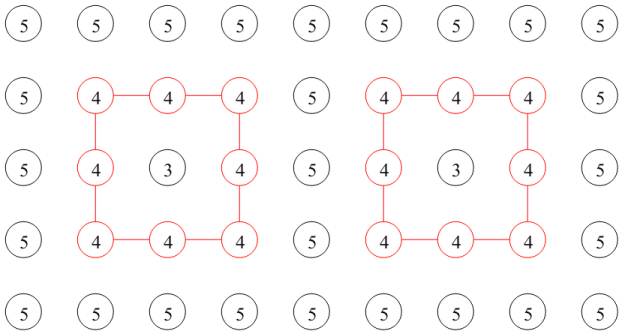
\includegraphics[height=5.5cm]{background/background-segmentation-levelsets-topologychanges-a.png}}%
	%
	\\ \vspace{4mm}%
	%
	\subfigure[Changing a single grid value merges the two components into one]
	{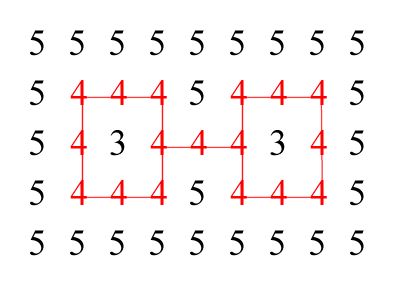
\includegraphics[height=5.5cm]{background/background-segmentation-levelsets-topologychanges-b.png}}%
\caption{Level set approaches seamlessly handle multiple boundaries and changes in topology}
\label{fig:background-segmentation-levelsets-topologychanges}
\end{stusubfig}
%---

Another advantage of level sets is that, unlike snakes, they translate straightforwardly into three dimensions -- all that is required is to replace a 2D grid with a 3D one. It is worth remarking, however, that the extra processing involved in the 3D case is substantial, making the basic scheme described above unsuitable if timely solutions are required. Special techniques have been developed to deal with this problem. One example is the narrow-band technique mentioned in \cite{malladi95}, which essentially restricts numerical calculations to a narrow region around the isosurface in which we're particularly interested (i.e.~the one representing the deformable model). The insight is that solving the PDE over the whole domain is only necessary if we're interested in solving for the entire family of isosurfaces associated with $\psi$: often, we're only interested in a single isosurface, so the extra computations aren't necessary. More details of this sort of technique are available in \cite{malladi95} and \cite{itk}.\fxnote{[IDV] [The level sets section needs an image-based example]}

An example illustrating the performance of a level set approach (the \emph{geodesic active contours} level set method from ITK, as described in \S9.3.3 of \cite{itk}) on an actual image is shown in Figure~\ref{fig:background-segmentation-levelsets-ct}. By carefully tweaking the (large number of) parameters to the method, it is possible to get very good results, making it an excellent technique for interactive segmentation. However, the requirement to provide so many parameters, whose effects on the results are not always intuitively obvious, makes the technique far less attractive as a method for more automatic segmentation.

%---
\begin{stusubfig}{p}
	\subfigure[The initial CT image, with seeds marked]
	{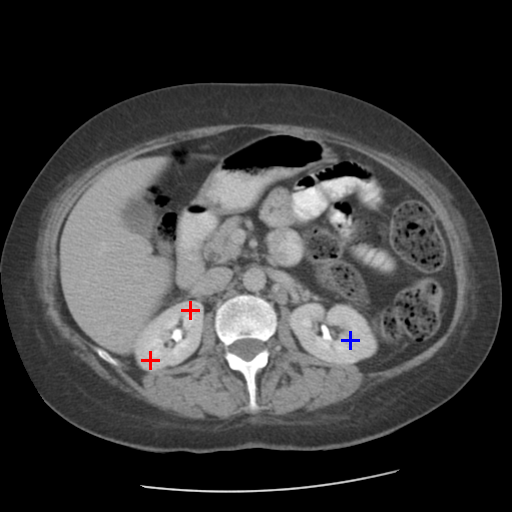
\includegraphics[height=5cm]{background/background-segmentation-levelsets-ct-a.png}}%
	%
	\hspace{4mm}%
	%
	\subfigure[The right kidney result]
	{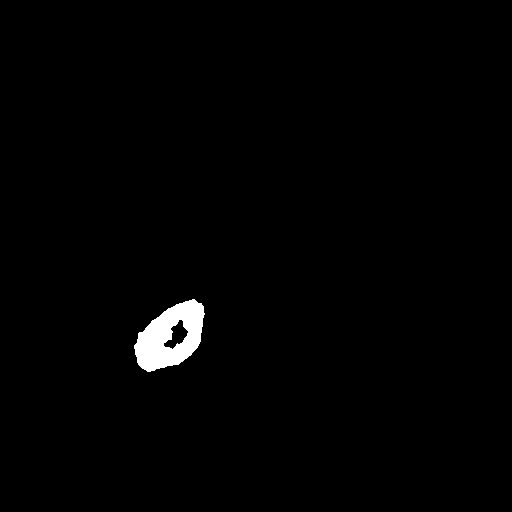
\includegraphics[height=5cm]{background/background-segmentation-levelsets-ct-b.png}}%
	%
	\\
	%
	\subfigure[The left kidney result]
	{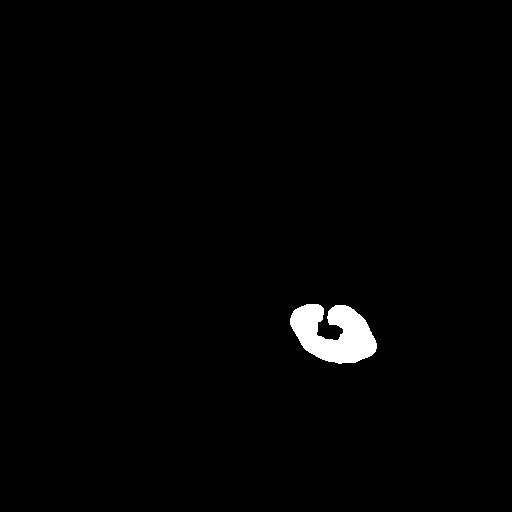
\includegraphics[height=5cm]{background/background-segmentation-levelsets-ct-c.png}}%
	%
	\hspace{4mm}%
	%
	\subfigure[Both results superimposed on the initial image]
	{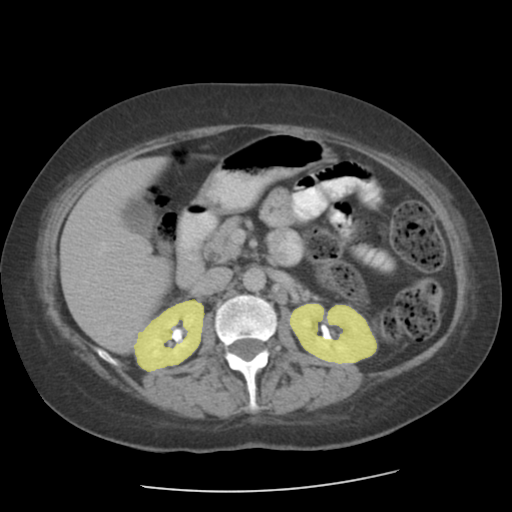
\includegraphics[height=5cm]{background/background-segmentation-levelsets-ct-d.png}}%
\caption{The results of using the \emph{geodesic active contours} level set method from ITK to identify kidneys in an example CT image. The (large number of) parameters had to be carefully tweaked by hand for each kidney, which is a downside of level set approaches.}
\label{fig:background-segmentation-levelsets-ct}
\end{stusubfig}
%---

%---
\stufigex{height=5.5cm}{background/background-segmentation-atlas-park.png}{Volume rendering of a probabilistic atlas constructed by Park et al.\ in \cite{park03} (extracted from Figure $2$ of the paper in question) -- the colours and brightnesses of the voxels depend on the probability values for the various organs at the voxels in question}{fig:background-segmentation-atlas-park}{p}
%---

%~~~~~~~~~~~~~~~~~~~~~~~~~~~~~~~~~~~~~~~~~~~~~~~~
\subsubsection{Other Deformable Models}
%~~~~~~~~~~~~~~~~~~~~~~~~~~~~~~~~~~~~~~~~~~~~~~~~

Although parametric and implicit models are the most common types of deformable model in use, there are some techniques which do not fall into either category. Two techniques in particular are worth briefly mentioning. In \cite{jalba04}, Jalba et al.\ use a deformable model based on charged particles to achieve some interesting automatic segmentation results. There, the model is represented neither parametrically nor implicitly, but instead as a set of charged particles under the influence of an electrostatic field. Another interesting type of deformable model is the m-rep, described by Pizer et al.\ in \cite{pizer03}. This uses a medial representation of the model.

%################################################
\subsection{Learning Techniques}
%################################################

Learning segmentation techniques generally start with a training phase, in which a large number of scans are taken and used to construct some variety of model, which encodes information that can be used to segment subsequent scans. Two different types of learning technique will be discussed in the following subsections.

%~~~~~~~~~~~~~~~~~~~~~~~~~~~~~~~~~~~~~~~~~~~~~~~~
\subsubsection{Atlas-Based Techniques}
%~~~~~~~~~~~~~~~~~~~~~~~~~~~~~~~~~~~~~~~~~~~~~~~~

Atlas-based methods start by constructing an atlas, or reference segmentation, from a set of training data. For instance, in \cite{park03}, Park et al.\ constructed a probabilistic atlas by registering (aligning) the manually segmented volumes of 31 patients onto that of a carefully chosen reference patient (thus the data came from 32 patients in all) -- see Figure~\ref{fig:background-segmentation-atlas-park} for a visual representation. The atlas was represented as a 3D grid of vector values, where the components of each vector corresponded to the organs under consideration, and the values of the components indicated the fractional percentage of registered data sets in which the point was labelled as the given organ. As an example, if we were considering the liver and the two kidneys, the vector $(0.4, 0.6, 0)^T$ at a point could indicate that the point was inside the liver in 40\% of the data sets and inside the right kidney in 60\% of them.

After constructing such an atlas, new sets of data can be segmented by registering them onto it. In \cite{park03}, they use a \emph{maximum a posteriori} (MAP) approach after registration to find the segmentation result which best explains the observed data. The important point here is that the segmentation result is based on both the data for the individual patient and the information encoded in the atlas. The atlas provides the prior probabilities at each voxel, and these are refined in light of the actual patient data.

To use the notation in \cite{park03}, we denote the segmentation result field as $\mathbf{X}$, the field of observed data for the individual patient as $\mathbf{Y}$, and the probabilistic atlas as $\mathbf{A}$. Each of these represents a volume of $N$ voxels, indexed linearly (in some order) from $1$ to $N$. So for instance, a particular segmentation result could be given by $\mathbf{x} = (x_1, x_2, \ldots, x_N)$. Our aim is to find the best possible $\mathbf{x}$, defined as
%
\[
\mathbf{\hat{x}} = \argmax_{\mathbf{x}} \mathbf{P}(\mathbf{X} = \mathbf{x} | \mathbf{Y} = \mathbf{y}).
\]
%
In other words, we seek the segmentation result which best explains the observed patient data, $\mathbf{y}$. The probabilistic atlas is used in all of this as the prior for $\mathbf{X}$. Suppose there are $L$ different possible voxel labels, numbered from $1$ to $L$. Each voxel $a_i$ of the probabilistic atlas contains an $L$-vector, $(a_{i,1}, \ldots, a_{i,L})$, where $a_{i,\ell}$ gives the probability of a voxel's correct label being $\ell$. We use this to define the prior probabilities for $\mathbf{X}$, writing
%
\[
P(x_i = \ell) = a_{i,\ell}.
\]
%
In other words, the probability of the correct segmentation result for a given voxel being $\ell$ is given by the $\ell^{th}$ component of the probabilistic atlas at that location. With this link made, the result determined will depend on both the atlas and the observed data.

%~~~~~~~~~~~~~~~~~~~~~~~~~~~~~~~~~~~~~~~~~~~~~~~~
\subsubsection{Neural Network Techniques}
%~~~~~~~~~~~~~~~~~~~~~~~~~~~~~~~~~~~~~~~~~~~~~~~~

Neural networks (NNs) can be used to segment images in a number of ways. A simple NN technique can be found in \cite{tsai94}, where Tsai and Tanahashi use a feed-forward network to classify each pixel into one of three classes (liver, boundary or non-liver) according to the grey-level histogram of the 7x7 region centred on the pixel. (In practice, they use a histogram with 16 grey levels instead of 256, to avoid a proliferation of input nodes in the NN.) The schematic of how this works (borrowed from their paper) is shown in Figure~\ref{fig:background-segmentation-neuralnets-tsai}. The NN is initially trained by picking a suitable image from the middle of the volume and marking a significant number of training regions for each class. The well-known back-propagation algorithm for NNs \cite{aima} is used to update the weights on the network arcs accordingly.

%---
\stufigex{height=20cm}{background/background-segmentation-neuralnets-tsai.png}{Schematic diagram of the neural-network-based boundary detection method used in \cite{tsai94} (reproduced from the paper in question)}{fig:background-segmentation-neuralnets-tsai}{p}
%---

A more up-to-date (and more complicated) NN scheme can be found in \cite{lee03}. Here, Lee et al.\ use a multi-module, recurrent neural network to segment multiple abdominal organs (see Figure~\ref{fig:background-segmentation-neuralnets-lee}). There is a module associated with each label under consideration. Each node of a given module $k$ corresponds to a pixel in the image and encodes the probability that the pixel should be assigned label $k$. The weights of the network arcs are initially derived from (for example) a correlation matrix containing the likelihoods of various labels occurring next to each other. (For example, the liver might be quite likely to occur next to the right kidney, but definitely shouldn't occur next to the left kidney.) An iterative state evolution algorithm is used to determine the probabilities at each node in each of the modules of the NN. The initial probabilities are generated using something called the `Kohonen self-organizing algorithm' (see the paper for details) and the nodes are updated at each time step based on the current probability at a given node and the support it receives from its neighbours. (So, for instance, if a pixel was currently classified as part of the left kidney, but all its neighbours were liver, it would be very likely to change to liver over time.) The results of this method (after combining it with fuzzy spatial rules for organ identification) are quite good -- see Figure~\ref{fig:background-segmentation-neuralnets-leeresults}.

%---
\stufigex{height=8cm}{background/background-segmentation-neuralnets-lee.png}{The architecture of the contextual neural network used in \cite{lee03} (reproduced from the paper in question)}{fig:background-segmentation-neuralnets-lee}{p}
%---

%---
\stufigex{height=8cm}{background/background-segmentation-neuralnets-leeresults.png}{Results of the neural network method described in \cite{lee03} (reproduced from the paper in question), showing the identified spine, left kidney, spleen and liver}{fig:background-segmentation-neuralnets-leeresults}{p}
%---

%~~~~~~~~~~~~~~~~~~~~~~~~~~~~~~~~~~~~~~~~~~~~~~~~
%\subsubsection{Statistical Methods}
%~~~~~~~~~~~~~~~~~~~~~~~~~~~~~~~~~~~~~~~~~~~~~~~~

%TODO: \cite{touhami05}

%################################################
\subsection{Clustering}
%################################################

Clustering is the general problem of how to collect objects into groups in such a way that the members of each group are (with relation to application-specific criteria) similar to each other, but dissimilar to those in other groups. This can evidently be applied to image segmentation, with the goal of clustering the image into groups of similar pixels.

%~~~~~~~~~~~~~~~~~~~~~~~~~~~~~~~~~~~~~~~~~~~~~~~~
\subsubsection{K-Means}
%~~~~~~~~~~~~~~~~~~~~~~~~~~~~~~~~~~~~~~~~~~~~~~~~

A generalised description of the K-means approach to clustering is that it aims to divide a set of $n$ objects $\{o_1,\ldots,o_n\}$ into $k \le n$ groups $G = \{G_1,\ldots,G_k\}$ in such a way as to minimise the sum of squares of some measure of similarity $m$ between each object and the `mean' of the objects of its group. (At this stage of the description, what is meant by the mean in this instance is left deliberately under-specified.) More formally, if $\mu_j$ is the mean of the objects in group $G_j$, K-means aims to find a set of groups $G$ minimising:
%
\[
\sum_{j=1}^k \sum_{o \in G_j} m(o, \mu_j)^2
\]
%
The method generally used to try and find $G$ is an heuristic known as Lloyd's algorithm \cite{lloyd82} (which, it must be remarked, may be difficult to discern from the original paper). This works as follows:

\begin{enumerate}

\item An initial set of $k$ means are chosen, either manually, randomly or otherwise.

\item Each object (in the case of imaging, each pixel) is assigned to the group to whose mean it is closest, i.e.~object $o$ is placed in the group with index:
%
\[
\argmin_{i=1}^k m(o, \mu_i)
\]

\item The means for all groups that have changed since the last iteration are recalculated.

\item Steps 2 and 3 are repeated until no groups change between one iteration and the next.

\end{enumerate}

\noindent Lloyd's algorithm is not guaranteed to find the global optimum for $G$, but it has been shown by Arthur and Vassilvitskii \cite{arthur07} that a careful choice of the initial means can make the algorithm $O(\log k)$-competitive with an optimal clustering (in other words, if the global optimum for $G$ is $G_{\mbox{OPT}}$, then the $G$ for the clustering produced by the algorithm satisfies $G / G_{\mbox{OPT}} \in O(\log k)$).

The key issues when using Lloyd's algorithm to segment images are how to define both the similarity measure and the mean of a set of pixels. One simple option is to define the similarity measure to be the absolute difference between pixel values, and the mean to be the average of the pixel values. (In other domains, the similarity measure might be the distance between objects, and the mean the average of the objects' positions.) This produces the sort of result shown in Figure~\ref{fig:background-segmentation-kmeans}. Whilst the result may appear superficially promising, it should be noted that the clusters produced by the K-means approach are not generally contiguous in the image (although some attempts have been made to address this in the literature, e.g.~see \cite{luo03,ilea06}). Furthermore, none of the clusters are really segmenting individual features, which is what we're most interested in. In practice, K-means segmentation is much better suited to segmentation tasks where there are a small number of well-defined pixel classes, e.g.~brain segmentation, where the goal is to separate the images into grey matter, white matter and cerebrospinal fluid. It is not especially well-matched to the problem of segmenting multiple abdominal organs with overlapping grey value distributions.

%---
\begin{stusubfig}{p}
	\subfigure[]
	{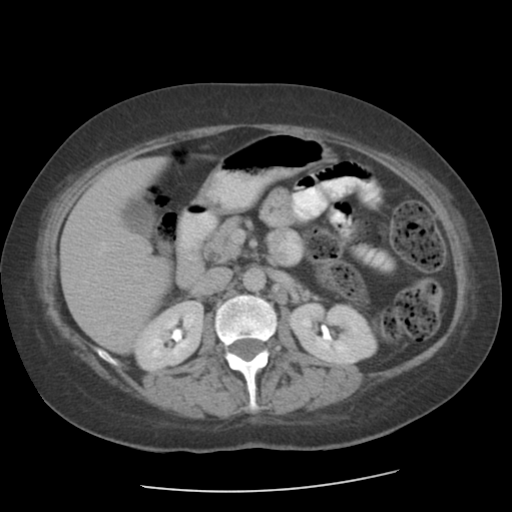
\includegraphics[width=.4\linewidth]{background/background-segmentation-kmeans-a.png}}%
	%
	\hspace{4mm}%
	%
	\subfigure[]
	{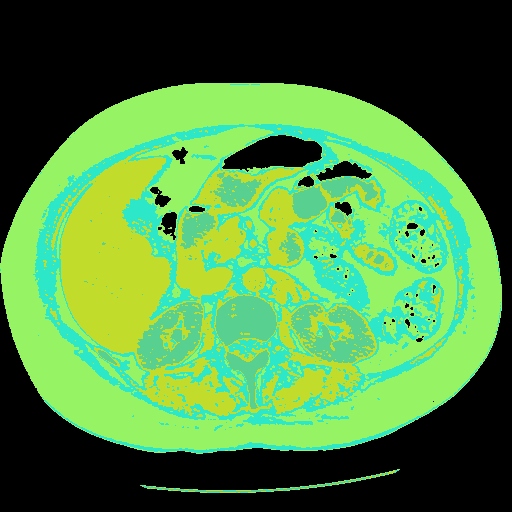
\includegraphics[width=.4\linewidth]{background/background-segmentation-kmeans-b.png}}%
\caption{An example of K-means clustering -- note that clustering the pixels of the example image (a) based on their values tends to produce non-contiguous clusters (b). For this example, the initial means chosen were $0$, $150$, $160$, $190$ and $255$.}
\label{fig:background-segmentation-kmeans}
\end{stusubfig}
%---

%~~~~~~~~~~~~~~~~~~~~~~~~~~~~~~~~~~~~~~~~~~~~~~~~
\subsubsection{Fuzzy C-Means}
%~~~~~~~~~~~~~~~~~~~~~~~~~~~~~~~~~~~~~~~~~~~~~~~~

Fuzzy C-means is essentially a fuzzy relative of the K-means approach just described. It was originally presented by Dunn in 1974 \cite{dunn74}. The key idea is that instead of objects being divided crisply into groups (i.e.~each object belonging completely to exactly one group), objects have a degree of membership for each group. Using the same notation as before, and letting $u_{ij}$ be a real number between $0$ and $1$ indicating the degree to which object $o_i$ is a member of group $G_j$, and $1 < p < \infty$ be a real parameter (e.g.~$p = 2$), we seek to find a set of groups $G$ minimising:
%
\[
\sum_{j=1}^k \sum_{o_i \in G_j} u_{ij}^p \cdot m(o,\mu_j)^2
\]
%
The standard algorithm for fuzzy C-means (as per \cite{matteucci}) is once again an iterative, heuristic method:

\begin{enumerate}

\item Initialise the $u_{ij}$ values for the first iteration (written as ${}^{(0)}u_{ij}$). Any of the initialisation approaches which work for K-means will work equally well for this (i.e.~it suffices to pick an initial set of means and assign objects completely to their nearest groups by setting the $u_{ij}$ value to $1$ for their group and $0$ for all other groups).

\item At iteration $s+1$, calculate the updated means of the groups using the equation:
%
\[
\mu_j^{(s+1)} = \frac{\displaystyle \sum_{o_i \in G_j} {}^{(s)}u_{ij}^p \cdot o_i}{\displaystyle \sum_{o_i \in G_j} {}^{(s)}u_{ij}^p}
\]

\item Calculate the updated values ${}^{(s+1)}u_{ij}$ using the equation:
%
\[
{}^{(s+1)}u_{ij} = \frac{1}{\displaystyle \sum_{n=1}^k \left( \frac{m(o_i, \mu_j^{(s)})}{m(o_i, \mu_n^{(s)})} \right)^{\frac{2}{p-1}}}
\]

\item Iterate Steps 2 and 3 until
%
\[
\max_{ij} |{}^{(s+1)}u_{ij} - {}^{(s)}u_{ij}| < \epsilon,
\]
%
where $\epsilon$ is a real number between $0$ and $1$.

\end{enumerate}

\noindent Once again, as with Lloyd's algorithm for K-means, this is not guaranteed to produce the global optimum.

%################################################
\subsection{Graph Partitioning}
\label{subsec:graphpartitioning}
%################################################

Graph partitioning segmentation algorithms work by representing an object to be segmented as a weighted, undirected graph. In the case of images, the nodes of this graph would be the pixels of the image, and each of its edges would connect a pair of adjacent pixels and be weighted according to some measure of the dissimilarity between those pixels (one possible definition, based on both the pixel values and their spatial location in the image, appears in \cite{shi00}). The idea is then to find a good way to partition the nodes of the graph into pieces. For instance, if $G = (V,E,w)$ is a graph with vertex set $V$, edge set $E$ and weight function $w$, the \emph{minimum cut} approach seeks to partition $V$ into two disjoint sets $A$ and $B$ such as to minimise:
%
\[
\mbox{cut}(A,B) = \sum_{u \in A, v \in B} w(u,v)
\]
%
As mentioned by (among others) Shi and Malik in \cite{shi00}, however, the minimum cut approach tends to partition the graph so as to cut away small groups of poorly connected nodes, with undesirable results. Instead, they define, and then try to minimise, a measure of the lack of quality of a binary partition called the \emph{normalized cut}, namely
%
\[
\mbox{Ncut}(A,B) = \frac{\mbox{cut}(A,B)}{\mbox{assoc}(A,V)} + \frac{\mbox{cut}(A,B)}{\mbox{assoc}(B,V)},
\]
%
where they define $\mbox{assoc}(X,V) = \sum_{u \in X, t \in V} w(u,t)$ for both $X = A$ and $X = B$. This solves the aforementioned problem with the minimum cut approach, because if (for example) $A$ is a small group of poorly connected nodes, we would expect $\mbox{cut}(A,B)$ to be almost the same as $\mbox{assoc}(A,V)$, leading to a large value for $\mbox{Ncut}(A,B)$.

Finding a good partition given the definition of a normalized cut involves solving an eigenvalue problem, the details of which are described in \cite{shi00}. Having solved the eigensystem, we\fxnote{[IDV] [Who is `we' here?]} take the second smallest eigenvector (for reasons discussed in the paper) and use it to try and compute a good partition. The eigenvector will have one real-valued component for each pixel in the image -- the idea is to find a splitting point which minimises the value of the normalized cut. Assuming the values are relatively well separated into two distinct clusters, this can be done by checking the cut value for a number of evenly-spaced, real-valued potential cut points, and picking the one with the lowest value. Pixels with values above the cut then form one group, and those with values below the other. If the values are not well separated, however, the cut values may well be similar for several different cut points. For that reason, \cite{shi00} defines a stability criterion which essentially measures the reliability of the cut.

The binary partitioning process thus far described then becomes part of a recursive partitioning scheme. Starting with the whole image, as good a binary partition as possible of the current image region is computed, along with the stability of the cut. If the stability is too low, the image region is not partitioned. Otherwise, the value of the cut itself is considered. If it is too high (i.e.~greater than some user-specified threshold), the recursion terminates. Otherwise, the binary partitioning process is repeated on the two sub-regions just computed. Via this recursive process, the image as a whole is partitioned into a number of groups dependent on the maximum allowed cut value and the stability criterion.

%################################################
\subsection{Hybrid Techniques}
%################################################

It is sometimes possible to achieve better results by combining a number of different segmentation methods than it is by using a single method on its own. A strikingly successful example of this sort of technique can be seen in the work of Luc Soler et al.\ \cite{soler01}, in which they describe an extensively hybrid technique for automatic segmentation of the liver from spiral CT scans. Their segmentation method first uses thresholding, morphological operators and distance maps to identify the skin, bones, lungs, kidneys and spleen. They next use a clever deformable model approach to embed a reference model of the liver into the image and automatically deform it to the liver contours. Later stages use Gaussian fitting on the image histogram to separate normal liver tissue from blood vessels and lesions (tumours), a result which is further refined by their own analytical methods. The final stage of their method makes use of higher-level medical knowledge to label the hepatic portal vein and segment the liver automatically according to an anatomically-based definition by Couinaud \cite{couinaud57}. The results of this technique are excellent -- see Figure~\ref{fig:background-segmentation-hybrid-soler}.

%---
\stufigex{height=8cm}{background/background-segmentation-hybrid-soler.png}{An automatic 3D reconstruction of patients from medical images, as performed by the IRCAD surgical planning tools developed using the work of Luc Soler et al.\ (the figure is reproduced from \cite{soler-imvie})}{fig:background-segmentation-hybrid-soler}{t}
%---

Other hybrid methods can be found in e.g.~\cite{ng06} and \cite{itk}. In \cite{ng06}, Ng et al.\ precede a watershed segmentation of MRI images of the head with a K-means clustering step -- this has the effect of hugely reducing the oversegmentation that the watershed would otherwise produce. It is a method that works particularly well for head segmentation, where the number of clusters is well-known a priori (in this case, the authors note that the types of tissue present tend to be `bone, soft tissue, fat and background'). There are several hybrid segmentation methods in \cite{itk}: in one, the authors combine fuzzy connectedness, Voronoi diagram classification and deformable models; in another, they combine Gibbs priors and deformable models. The details of these techniques are beyond the scope of this dissertation, but an implementation of the methods can be found in the freely-available \emph{Insight Toolkit} \cite{itk}.\fxnote{[IDV] [This needs a reference]}

\fxnote{[IDV] I'd put a section/paragraph on ITK here}

\clearpage

%##################################################################################################
\section{Partition Hierarchies}
\label{sec:background-partitionhierarchies}
%##################################################################################################

%TODO: (i) Brief description of what a partition tree is; (ii) Explain, with suitable references, the various situations in which they are used; (iii) Narrow it down to images and survey the various techniques, noting the key differences between the representations (e.g.~whether or not adjacency information is maintained, etc.); (iv) Explain (at a high level) how partition forests fit into the picture

%################################################
\subsection{Overview}
%################################################

Partition\fxnote{[IDV] Define `partition'} hierarchies comprise two related data structures -- partition trees and partition forests. A \emph{partition tree} is a tree-based data structure containing nodes that represent portions of an entity, and satisfying the condition that the sub-entities represented by the children of any node in the tree partition the sub-entity represented by that node -- that is, the child sub-entities together form the parent sub-entity, and none of the child sub-entities mutually overlap. (I will henceforth, for reasons of brevity, refer to nodes partitioning each other, rather than referring to the sub-entities they represent.) An example of a partition tree can be seen in Figure~\ref{fig:background-partitionhierarchies-treeexample}. Partition forests will be discussed below (and in Chapter~\ref{chap:ipfs}).

%---
\stufigex{height=9cm}{background/background-partitionhierarchies-treeexample.png}{A partition tree for the set $\{a,b,c,d,e\}$ -- note that the sets represented by child nodes partition the set represented by their parent, e.g.~$\{c\}$ and $\{d,e\}$ partition $\{c,d,e\}$.}{fig:background-partitionhierarchies-treeexample}{p}
%---

Partition trees can be either incomplete or complete. An incomplete partition tree is one with an incomplete lowest layer (as in Figure~\ref{fig:background-partitionhierarchies-treeexample}), and a complete one is the opposite. Complete partition trees have the property that the nodes in any given layer form a partition of the entity as a whole. For either type of tree, this is also true of the set of leaf nodes (those nodes without children). It should be noted that every incomplete partition tree has an equivalent complete partition tree. This can be constructed by adding a chain of nodes downwards from every leaf which is not in the lowest layer -- see Figure~\ref{fig:background-partitionhierarchies-completetree} for a complete tree corresponding to the incomplete tree we've seen so far.

%---
\stufigex{height=9cm}{background/background-partitionhierarchies-completetree.png}{A \emph{complete} partition tree corresponding to the incomplete one in Figure~\ref{fig:background-partitionhierarchies-treeexample}}{fig:background-partitionhierarchies-completetree}{p}
%---

There are essentially two ways of constructing partition trees -- top-down or bottom-up. Top-down approaches start with a root node representing the entire entity, and recursively split it until some desired termination criteria are satisfied. Bottom-up approaches, by contrast, start with a partition of the entity into the smallest sub-entities possible. One common bottom-up approach makes this partition the lowest layer of the tree, then iteratively (a) clones the current highest layer of the tree and (b) merges some of the nodes in it together. The process terminates when the highest layer of the tree contains exactly one node (the root). Note that this technique naturally produces complete partition trees. An alternative bottom-up approach is to iteratively merge pairs of nodes together: this produces a data structure known as a dendogram, which is an incomplete tree (even if it is sometimes depicted graphically with all its leaves in a single layer). Whilst top-down approaches can also theoretically produce complete partition trees, they tend not to in practice. When bottom-up approaches are terminated early (i.e.~whilst the highest layer still contains more than one node), they construct not a partition tree, with a single root, but a forest of such trees (which can naturally be called a \emph{partition forest}). I have devised a number of novel algorithms for working with partition forests, and these are the subject of Chapter~\ref{chap:ipfs}.

Since representing entities hierarchically is a fundamental way in which we, as humans, seek to manage the inherent complexity of the world around us, partition hierarchy usage is fairly common in computer science. The varied contexts in which partition hierarchies can be used, to name but a few, include image representation, hierarchical pathfinding, and world representation. World representation, whilst a fascinating topic in its own right, is sadly somewhat outside the scope of this dissertation, but the interested reader can find a detailed description of one approach to it (binary space partitioning, as originally presented in \cite{fuchs80}) in the appendices of my undergraduate project report \cite{golodetz06}. Hierarchical pathfinding, somewhat surprisingly, is more relevant, in that it provides a direct application for the partition forest algorithms I describe in Chapter~\ref{chap:ipfs}. For that reason, both image representation and hierarchical pathfinding are now discussed in more detail.

%################################################
\subsection{Image Representation}
%################################################

The `grid-of-pixels' representation of images is by far the most familiar, but it contains fine-grained information at the expense of structure. This makes it less than ideal for image processing tasks such as feature identification, for which structure in the image is important. For this reason, there has long been a great deal of research interest in representing images hierarchically (for example, images were being represented as quadtrees at least as far back as the 1970s \cite{klinger76} and 1980s \cite{ahuja83,samet80}). Hierarchical representations recursively group the pixels into larger regions -- the idea in terms of feature identification is to construct a hierarchy in which the regions are actually meaningful in the problem domain (essentially the problem segmentation algorithms aim to solve). Feature identification algorithms can then work at the level of the regions in the hierarchy, which ideally correspond much better to the actual features we are trying to identify.

One hierarchical representation is the binary partition tree (BPT), originally described by Salembier and Garrido in \cite{salembier00}. A BPT is an incomplete, binary tree containing limited region adjacency information (each node is implicitly connected to its sibling). The construction process described in \cite{salembier00} starts from an initial partition and iteratively merges pairs of adjacent regions in increasing order of dissimilarity. The result of each merge becomes a region which is then considered with the rest. (The process thus constructs a dendogram.) The algorithm terminates when either a single region, or a user-specified number of regions, remains. Descriptors (properties) can be assigned to each node, and the descriptor of a parent node can often be calculated from those of its children. These descriptors can then be used by feature identification algorithms. BPTs have seen use in e.g.~\cite{cooray01,salembier02}. The original BPT framework is easily customisable, in the sense that different trees can be created by using a different region similarity criterion (thus altering the merging order) and termination criterion. In \cite{bennstrom04}, Bennstr\"om et al.\ defined a so-called `quasi-inclusion' criterion for region similarity that orders regions for merging based on the extent to which they are contained within each others' convex hulls. The corresponding termination criterion simply specifies a quasi-inclusion threshold: for instance, that merging should continue until all the regions that are at least 50\% contained within another region's convex hull have been merged. In \cite{al-haj08}, Al-Haj and Al Aghbari essentially define yet another alternative merging order for colour image segmentation via the use of spatio-visual grouping rules, calling the result a `semantic segmentation tree'.

An alternative hierarchical representation, and one which is of key interest for the purposes of this dissertation, is what I call an image partition forest \cite{gvccimi08,gvcispa09}. This has appeared under a variety of other names in the literature: among others, hierarchy of (region adjacency) graphs \cite{kropatsch04,nacken95,shen97}, hierarchical attributed region adjacency graph \cite{fischer04}, hierarchy of partitions \cite{haxhimusa03,lezoray06}, picture tree \cite{andrade03}, graph pyramid \cite{kerren06}, bounded irregular pyramid \cite{marfil07} and segmentation graph \cite{borenstein06}. (It has also appeared as a hierchical image representation with no specific name, e.g.~\cite{qimin04,yu02}.)

An image partition forest is a complete (i.e.~its lowest layer is complete), n-ary forest. It is constructed using the bottom-up approach that takes an initial partition and then iteratively (a) clones the highest layer and (b) merges some of the regions in it. The way in which regions are chosen to merge in each layer varies between approaches. In my work I used the waterfall transform \cite{marcotegui05} for this, which essentially performs a watershed transform to segment the region adjacency graph of the current highest layer, but any number of other methods are possible: for instance, the algorithm in \cite{yu02} takes the current highest layer, merges neighbouring regions whose similarity measure is below a given threshold, and then merges any singleton regions with their nearest neighbour. As with BPTs, region properties can be assigned to each node and used for later feature identification.

Despite the widespread use of the partition forest data structure, comparitively little research appears to have been done into ways of editing partition forests after they have been constructed. One key paper which did look at this area is \cite{nacken95}, in which Nacken discusses an approach to what he calls connectivity-preserving relinking -- the problem I have tackled as parent switching (or how to change the hierarchy so as to move a node from being the child of one parent to being the child of another). Nacken's approach is to identify the two cases in which a node cannot be moved between parents: (1) when the node is not adjacent to its new parent and (2) when moving the node would divide its old parent. He then prevents nodes being moved if either case occurs. I independently identified the same two cases in my own work, but, rather than preventing a node being moved in case (2), my approach essentially splits the remainder of the old parent and any ancestors (where necessary) into their connected components to maintain consistency in the hierarchy. This could be considered a more flexible approach than Nacken's, in that it allows a greater number of possible moves. To the best of my knowledge, the other partition forest algorithms I will present, such as unzipping, zipping and non-sibling node merging, have no comparisons in the literature.

%################################################
\subsection{Hierarchical Pathfinding}
%################################################

As is well-known among computer scientists, the basic pathfinding problem over graphs, that of finding the shortest route from one node to another in a weighted graph, can in principle be `solved' using common algorithms such as Dijkstra's or, more usually, A* \cite{aima}. However, in domains with hard real-time constraints (such as AI for computer games \cite{dickheiser04,vandersterren04}, in which it is often necessary for large numbers of pathfinding queries to be resolved in an extremely short space of time, or traffic guidance systems \cite{jing96,jung96,kim98}, where drivers need real-time route updates to help them avoid congestion), pathfinding using these algorithms can take an unacceptably long time. An alternative, if the graph is static, is to precompute the best paths between all pairs of nodes in the graph offline and store them in a transition table (see Figure~\ref{fig:background-partitionhierarchies-pathfinding-transitiontable}). However, this rapidly becomes impractical for even moderately-sized graphs, as it requires a quadratic amount of storage.

%---
\begin{stusubfig}{p}
	\subfigure[]
	{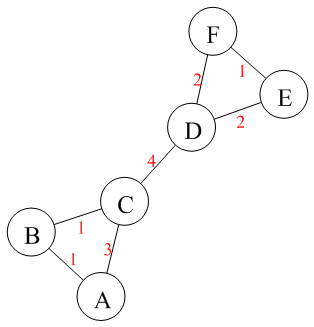
\includegraphics[height=6cm]{background/background-partitionhierarchies-pathfinding-transitiontable-a.png}}%
	%
	\hspace{4mm}%
	%
	\subfigure[]
	{
	\raisebox{1cm}{\begin{tabular}[b]{cc|cccccc}
	&& \multicolumn{6}{c}{Destination} \\
	&& A & B & C & D & E & F \\
	\hline
	\multirow{6}{*}{Source}
	& A  & $\times$ & B & B & B & B & B \\
	& B  & A & $\times$ & C & C & C & C \\
	& C  & B & B & $\times$ & D & D & D \\
	& D  & C & C & C & $\times$ & E & F \\
	& E  & D & D & D & D & $\times$ & F \\
	& F  & D & D & D & D & E & $\times$
	\end{tabular}}
	}%
\caption{A graph and its corresponding transition table -- each table entry $t_{SD}$ stores the node after $S$ on the optimal path between $S$ and $D$}
\label{fig:background-partitionhierarchies-pathfinding-transitiontable}
\end{stusubfig}
%---

Hierarchical pathfinding is an approach designed to reduce these prohibitive storage costs. The essence of the idea is to partition the graph into clusters. This partitioning of the graph into clusters creates a two-layer partition hierarchy (in this case a partition forest) of the graph nodes. Pathfinding schemes can then be devised that still produce optimal paths, but only store the substantially smaller transition tables for paths within each cluster and a transition table for an inter-cluster `super-graph' -- for an illustration of this sort of scheme, see Figure~\ref{fig:background-partitionhierarchies-pathfinding-kim}. The kind of storage savings that can be expected from this sort of approach are quantified by Dickheiser in \cite{dickheiser04}.

%---
\stufigex{height=10cm}{background/background-partitionhierarchies-pathfinding-kim.png}{Partitioning a large graph into clusters allows us to only store transition tables for each cluster (b) and the super-graph (c), rather than a transition table for the entire graph. When finding paths, all the necessary information is contained in the transition tables for the source cluster, the destination cluster and the super-graph (d). (The figure is reproduced from Kim et al.\ \cite{kim98}.)}{fig:background-partitionhierarchies-pathfinding-kim}{p}
%---

To find an optimal path between two nodes using this scheme, we observe that such a route can either (a) go from the source node to a boundary node of the source cluster, then (via the super-graph) to a boundary node of the destination cluster, then to the destination node, or (b) go directly from the source node to the destination node if they are in the same cluster. (Note that the shortest path between two nodes in the same cluster may actually go via the super-graph, so we have to consider both options in such a case.) An optimal intra-cluster route (where applicable) can simply be looked up in the cluster's transition table, but to find an optimal inter-cluster route is slightly more involved. To do so, we find three sets of optimal sub-paths:
%
\begin{enumerate}

\item $S = \{s_i\}$, the set of optimal paths from the source node to a boundary node of the source cluster. These can be looked up using the source cluster's transition table.
\item $P = \{p_j\}$, the set of optimal paths from a boundary node of the source cluster to a boundary node of the destination cluster. These can be looked up using the super-graph's transition table.
\item $D = \{d_k\}$, the set of optimal paths from a boundary node of the destination cluster to the boundary node. These can be looked up using the destination cluster's transition table.

\end{enumerate}
%
We then consider all possible paths $s_i \mbox{++} p_j \mbox{++} d_k$ (where $\mbox{++}$ represents path concatenation) and pick one with the lowest cost. This is minimised against any possible intra-cluster route where necessary to give a path that is optimal overall.

Thus far, we have only considered a pathfinding hierarchy with two layers, but the scheme can easily be extended to allow more layers if e.g.~the transition tables for the individual clusters are still considered too memory-intensive. The easiest way to do this is to treat each individual cluster as a graph in its own right and partition it into pieces (a top-down approach), although bottom-up approaches are also possible (one such approach, referred to in \cite{kim98}, can be found in \cite{jing96}). Actually constructing the partitions of individual graphs automatically is the problem known as graph partitioning or graph clustering (see e.g.~\cite{huang96,jing98}, or indeed \S\ref{subsec:graphpartitioning}). In certain domains (such as the computer games industry), the partitions may actually be constructed manually to gain finer control over the end result \cite{dickheiser04}. In either case, however, it is helpful to be able to edit the resulting partition forest interactively to try and minimise the amount of memory required to store the transition tables. This can be facilitated by the partition forest algorithms I will present in Chapter~\ref{chap:ipfs}.

%##################################################################################################
\section{Chapter Summary}
%##################################################################################################

This chapter has given an overview of most of the techniques currently in use for medical image segmentation and provided some important background on the varied uses of partition hierarchies. In Chapter~\ref{chap:methodology}, I will discuss the design of my research in the context of these large bodies of existing work.
